\documentclass{book} % Definisi jenis dokumen

%%%%% Definisi paket-paket yang wajib digunakan %%%%%
\usepackage[utf8]{inputenc} % paket encoding input utf8 (wajib)
\usepackage[T1]{fontenc} % paket encoding huruf latin (wajib)

%%%%% Definisi paket-paket yang digunakan sesuai kebutuhan %%%%%
\usepackage[yyyymmdd,hhmmss]{datetime} % paket tanggal-waktu
\usepackage{graphicx} % paket grafik/gambar
\usepackage[english]{babel} % paket modifikasi label/caption pada bahasa tertentu
\usepackage{geometry} % paket ukuran kertas dan margin
\usepackage{hyperref} % paket referensi url dan hyperref
\usepackage{minted} % paket lingkungan kode sumber
\usepackage{xcolor} % paket definisi warna
\usepackage[os=win]{menukeys} % paket simbol keyboard standard Windows

%%%%% Pengaturan ukuran kertas dan margin %%%%%
\geometry{
	a4paper,
	left=10mm,
	right=10mm,
	top=15mm,
	bottom=15mm,
}

%%%%% Pengaturan perintah informasi perangkat lunak %%%%%
\newcommand{\ShowOsVersion}{
	\immediate\write18{\unexpanded{foo=`uname -sro` && echo "${foo}" > tmp.tex}}
	\input{tmp}\immediate\write18{rm tmp.tex}
}

\newcommand{\ShowTexVersion}{
	\immediate\write18{\unexpanded{foo=`pdflatex -version | head -n1 | cut -d' ' -f1,2` && echo "${foo}" > tmp.tex}}
	\input{tmp}\immediate\write18{rm tmp.tex}
}

%%%%% Mengganti label "Contents" ke "Daftar Isi" %%%%%
\addto\captionsenglish{\renewcommand{\contentsname}{Daftar Isi}}

%%%%% Mengganti label "Figure" ke "Gambar" %%%%%
\addto\captionsenglish{\renewcommand{\figurename}{Gambar}}

%%%%% Pengaturan teks link url/hyperref %%%%%
\hypersetup{
	colorlinks=true, %set true if you want colored links
	linktoc=all,     %set to all if you want both sections and subsections linked
	linkcolor=blue,  %choose some color if you want links to stand out
	urlcolor=blue,   %url color
}

%%%%% Definisi warna baru %%%%%
\definecolor{LightGray}{gray}{0.95}

\begin{document}

    %%%%%%%%%%%%%%%%%%%%%%%%%%%%%%%%%%%%%%%%%%%%%%%%%%%%%%%%%%%%%%%%%

    \frontmatter % untuk halaman cover

    \begin{titlepage}
        \centering % untuk membuat tengah teks

        {
            \LARGE % pakai font besar
            \bf % pakai font BOLD
            Pengenalan LaTeX untuk Pemula
        }

        {\Large \bf Achmadi ST MT}
        \vfill % menambahkan ruang kosong vertikal

		
\includegraphics[width=500pt]{images/leafcover}
		\vfill

		\raggedright
		\noindent Buku ini ditulis dengan:\\ % tanda \\ menambahkan garis baru
		OS : \ShowOsVersion \\
		TeX : \ShowTexVersion \\
		Update: {\today} at \currenttime\\
    \end{titlepage}

	%%%%%%%%%%%%%%%%%%%%%%%%%%%%%%%%%%%%%%%%%%%%%%%%%%%%%%%%%%%%%%%%%

	\newpage % halaman baru

	\tableofcontents % daftar isi

	%%%%%%%%%%%%%%%%%%%%%%%%%%%%%%%%%%%%%%%%%%%%%%%%%%%%%%%%%%%%%%%%%

    \newpage
    \chapter{Disclaimer} % memulai chapter baru

    LaTeX adalah proyek typesetting yang dimulai oleh \href{https://en.wikipedia.org/wiki/Leslie_Lamport}{Leslie Lamport}
    sekitar 40 tahun lalu dan sekarang dilanjutkan oleh \href{https://www.latex-project.org/}{latex-project.org}.

    \bigskip % baris kosong pemisah paragraf

    Buku tutorial ini disarikan dari \href{https://latex-tutorial.com/tutorials}{latex-tutorial.com}
    dan \href{https://www.overleaf.com/learn/latex/Tutorials}{overleaf.com} dengan alih bahasa dan penambahan konten sesuai selera penulis.

    %%%%%%%%%%%%%%%%%%%%%%%%%%%%%%%%%%%%%%%%%%%%%%%%%%%%%%%%%%%%%%%%%

	\newpage
	\chapter{Penggunaan Buku}

	\section{Umum} % memulai section baru
	Buku ini dibuat dengan tujuan penggunaan utama sebagai panduan digital untuk mempermudah search dan copy-paste.
	Anda tidak perlu mencetak buku ini ke bentuk kertas.
	Seluruh navigasi buku ini diharapkan menggunakan klik ke hyperlink di Daftar Isi,
	atau menggunakan tampilan \textbf{Index} yang tersedia di \textbf{SideBar} program pembaca PDF yang anda gunakan.

	\section{Petunjuk}
	Beberapa petunjuk yang digunakan di buku ini:
	\begin{itemize} % memulai lingkungan daftar tanpa angka (bullet list)
		\item \textbf{Cetak Tebal}: Menginformasikan identifier (keyword, opsi, nama file, dst) yang berada di suatu paragraf
		\item \textit{Cetak Miring}: Bersama simbol panah (->) dan simbol lain, menginformasikan langkah-langkah klik menu/tombol.
		\item \textbf{TIPS:} Menginformasikan hal-hal yang dapat membantu atau pengetahuan tambahan.
		\item \textbf{PERINGATAN:} Menginformasikan hal-hal yang bener-benar harus diperhatikan.
	\end{itemize}

	\section{Penulisan Kode}
	Untuk penulisan kode, akan digunakan sebagai berikut:

    % lingkungan penulisan kode sumber
    \begin{minted}[frame=lines,framesep=2mm,fontsize=\normalsize,bgcolor=LightGray]{latex}
\begin{enumerate}
    \item Pertama
    \item Kedua
\end{enumerate }
    \end{minted}

    \section{Kode Sumber Dokumen}

    Seluruh isi buku ini juga ditulis dengan LaTeX, sehingga jika dibutuhkan contoh, dapat melihat
    kode sumber dokumen ini yang tersedia di \href{https://github.com/mekatronik-achmadi/my_latexbook/blob/master/Modul/LaTex/latex_beginner.tex}{GitHub}.

    \bigskip

    Selain itu, website seperti \href{https://www.overleaf.com/}{Overleaf.com} menyediakan beragam tutorial dan contoh siap pakai.

    %%%%%%%%%%%%%%%%%%%%%%%%%%%%%%%%%%%%%%%%%%%%%%%%%%%%%%%%%%%%%%%%%

    \mainmatter % pindah format halaman dari romawi ke angka (konten utama)

    \newpage
    \chapter{Introduksi}

    \section{Apa itu LaTeX}

    LaTeX adalah bahasa markup (seperti HTML dan Markdown) untuk typeset (mengatur penulisan) dokumen.
    Format berkas dokumen LaTeX umumnya berupa berkas teks yang disimpan di suatu folder
    bersamaan dengan berkas pendukung lain (seperti gambar, pdf, dan sebagainya).
    Berkas teks ini kemudian dikompilasi menjadi berkas akhir (umumnya PDF atau DVI).

    LaTeX sangat populer digunakan untuk antara lain:
    \begin{itemize}
        \item Jurnal, paper, atau artikel akademik.
        \item Laporan Teknis.
        \item Buku atau Novel.
        \item Presentasi.
    \end{itemize}

    \section{Contoh kode LaTeX}

    Berikut contoh kode LaTeX untuk menulis tabel:

    \begin{minted}[frame=lines,framesep=2mm,fontsize=\normalsize,bgcolor=LightGray]{latex}
\begin{center}
    \begin{tabular}{ |c|c|c| }
        \hline
        cell1 & cell2 & cell3 \\
        \hline
        cell4 & cell5 & cell6 \\
        \hline
        cell7 & cell8 & cell9 \\
        \hline
    \end{tabular}
\end{center}
    \end{minted}

    Hasil kode di atas akan menghasilkan sebagai berikut:
    \begin{center}
        \begin{tabular}{ |c|c|c| }
            \hline
            cell1 & cell2 & cell3 \\
            \hline
            cell4 & cell5 & cell6 \\
            \hline
            cell7 & cell8 & cell9 \\
            \hline
        \end{tabular}
    \end{center}

    \section{Komentar dalam LaTeX}

    Selayaknya bahasa pemrograman pada umumnya, LaTeX mengenal mekanisme komentar yang tidak akan dikompilasi ke dokumen akhir.
    Komentar dalam latex adalah komentar per baris yang dimulai dengan karakter persen '\%'.

    Sebagai contoh:

    \begin{minted}[frame=lines,framesep=2mm,fontsize=\normalsize,bgcolor=LightGray]{latex}
\begin{itemize}
    \item First % Ini pertama
    \item Second % Ini kedua
\end{itemize}
    \end{minted}

    Yang akan menghasikan (tanpa ada konten setelah tanda persen) :

    \begin{itemize}
        \item First % Ini pertama
        \item Second % Ini kedua
    \end{itemize}

    Jika dibutuhkan menulis simbol persen, ditambahkan simbol backslash ('\textbackslash').
    Contohnya:

    \begin{minted}[frame=lines,framesep=2mm,fontsize=\normalsize,bgcolor=LightGray]{latex}
Uang senilai 50\% dari Rp.1000 adalah Rp.500
    \end{minted}

    Menghasilkan: \\
    Uang senilai 50\% dari Rp.1000 adalah Rp.500

    \section{Apakah LaTeX termasuk Word-Processor}

    LaTeX sama sekali \textbf{BUKAN} word-processor seperti MS-Word, LO-Writer, OO-Document, Google-Doc, atau yang serupa.

    \bigskip

    Perbedaan mendasar adalah:
    \begin{itemize}
        \item Word-Processor menganut paradigma WYSIWYG,
        sedangkan LaTeX adalah markup dan typesetting yang perlu dikompilasi terlebih dahulu.

        \item Word-Processor modern membutuhkan perangkat layout seperti mouse/touchpad,
        sedangkan LaTeX murni programmatikal teks.
    \end{itemize}

    \bigskip

    Keuntungan Word-processor dibandingkan LaTeX:
    \begin{itemize}
        \item Dokumen workflow yang telah dikenalkan sejak kita SD.
        \item Penguna lebih banyak dan lebih umum.
    \end{itemize}

    \bigskip

    Keuntungan LaTeX dibandingkan Word-Processor:
    \begin{itemize}
    	\item Format dan paket LaTeX bersifat gratis dan open-sources.
        \item Satu template dapat digunakan berkali-kali.
        \item Tampilan dokumen diatur template, sehingga penulis bisa fokus pada konten saja.
        \item Hasil penulisan format rumus kompleks bagus.
        \item Hasil penulisan kode programming bagus.
        \item Hasil penulisan bibliografi akademik bagus.
        \item Format berkas adalah teks, sehingga mudah untuk editting (tidak butuh CPU/GPU/RAM besar)
        dan dapat direkam content-tracking atau source-code manager seperti Git, CVS, atau Mercurial.
    \end{itemize}

	%%%%%%%%%%%%%%%%%%%%%%%%%%%%%%%%%%%%%%%%%%%%%%%%%%%%%%%%%%%%%%%%%

	\chapter{Installasi}

	Mengingat LaTeX yang bersifat open-sources, maka dapat dipastikan LaTeX tersedia di major-OS seperti GNU/Linux, Windows, dan MacOS.
	Selain paket offline, tersedia pula LaTeX editor dan builder online.

	\section{Paket Offline}

	Keuntungan instalasi paket offline antara lain:

	\begin{itemize}
		\item Tidak selalu membutuhkan koneksi internet.
		\item Kompilasi PDF cenderung lebih cepat.
		\item Modifikasi dan pengaturan dapat permanen.
	\end{itemize}

	\subsection{GNU/Linux}

	\subsubsection{TexLive}

	Distribusi LaTeX yang saat ini (tahun 2022) umum digunakan adalah \href{https://www.tug.org/texlive/}{TeX LIve}.
	Distribusi ini telah tersedia di banyak distro GNU/Linux dan dapat diinstall dari repository masing-masing melalui perintah di terminal.
	Konsultasikan dengan admin GNU/Linux anda jika kesulitan menginstal.

	Contoh instalasi disini akan digunakan contoh pada ArchLinux/Manjaro, namun umumnya serupa untuk distro OS GNU/Linux lain seperti Ubuntu atau Fedora.

	Perintah di terminal untuk instalasi:
	\begin{minted}[frame=lines,framesep=2mm,fontsize=\normalsize,bgcolor=LightGray]{bash}
$> sudo pacman -S texlive-formatsextra texlive-bibtexextra \
texlive-latexextra texlive-publishers texlive-fontsextra \
texlive-pictures texlive-pstricks texlive-science texlive-core \
texlive-bin latex2html latex2rtf dblatex minted biber pdftk
	\end{minted}

	Untuk paket penuh lengkap akan mendownload setidaknya 800MB dan instalasi sekitar 2.5GB.

	\bigskip

	Kemudian untuk pilihan editor, berikut tersedia beberapa pilihan

	\subsubsection{TexStudio}

	TexStudio adalah lingkungan terintegrasi untuk mengerjakan dokumen LaTeX.
	TexStudo bersifat gratis dan open-sources.
	Fitur utama TexStudio antara lain:
	\begin{itemize}
		\item Syntax-Highlighting.
		\item Cek Reference/Bibliography.
		\item Auto-Completion yang sangat lengkap.
	\end{itemize}

	Perintah instal di terminal:

	\begin{minted}[frame=lines,framesep=2mm,fontsize=\normalsize,bgcolor=LightGray]{bash}
$> sudo pacman -S texstudio
	\end{minted}

	Instalasi akan berkisar 500MB (ditambah instalasi pustaka Qt5 sebagai toolkit GUI).

	\newpage
	\begin{figure}[!ht]
% lingkungan untuk gambar
		\centering
		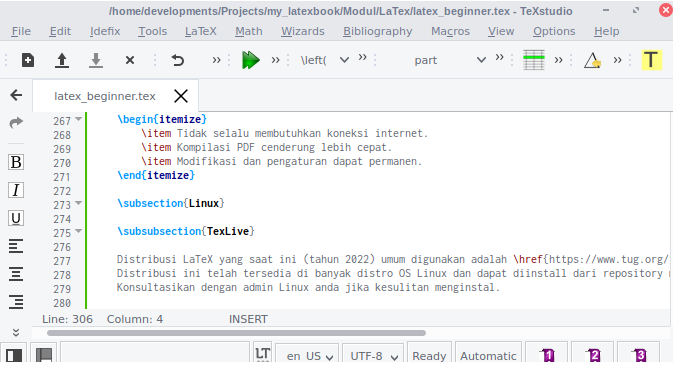
\includegraphics[width=400pt]{images/texstudio}
		\caption{Contoh TexStudio}
	\end{figure}

	\textbf{TIPS:} Untuk perintah kompilasi, pastikan terdapat opsi \textbf{-shell-escape}.
	Jika belum, dapat ditambahkan opsi tersebut pada menu \textit{Options} -> \textit{Configure TexStudio}.
	Kemudian pilih tab \textit{Commands}.

	\begin{figure}[!ht]
% lingkungan untuk gambar
		\centering
		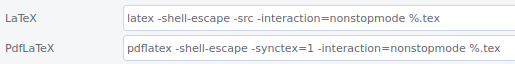
\includegraphics[width=450pt]{images/texstudio_shellescape}
		\caption{Opsi Shell Escape}
	\end{figure}

	\subsubsection{Visual Studio Code}

	Visual Studio Code adalah editor pemrograman multiguna buatan Microsoft yang fungsi dan fiturnya dapat ditambahkan dengan segudang ekstensi.
	Untuk mengerjakan LaTeX, dapat digunakan ekstensi \href{https://github.com/James-Yu/LaTeX-Workshop}{LaTeX-Workshop}.

	Untuk instalasi di ArchLinux/Manjaro, dapat digunakan paket VSCodium di AUR:\\
	\url{https://aur.archlinux.org/packages/vscodium-bin/}.

	\begin{figure}[!ht]
		\centering
		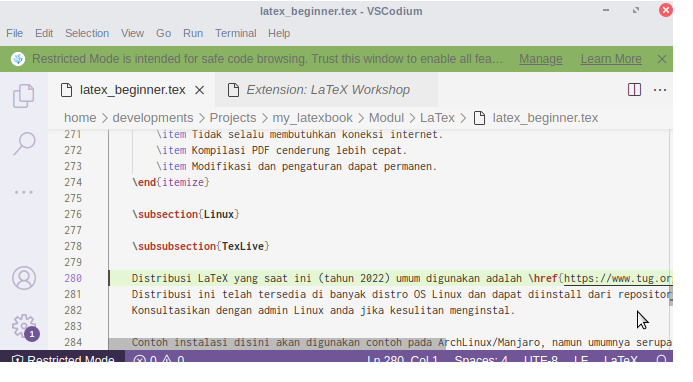
\includegraphics[width=400pt]{images/vscodium}
		\caption{Contoh VSCodium}
	\end{figure}

	Kemudian ekstensi LaTeX Workshop dapat diinstal di program VSCodium sendiri pada menu \textit{View} -> \textit{Extension}.

	\newpage

	\subsubsection{Makefile}

	Khusus GNU/Linux, pada dasarnya dapat digunakan editor teks apapun (termasuk editor CLI seperti Vim, Nano, atau Emacs).
	Untuk mengkompilasi berkas LaTeX (umumnya berekstensi \textbf{*.tex}), dapat digunakan perintah di terminal seperti:

	\begin{minted}[frame=lines,framesep=2mm,fontsize=\normalsize,bgcolor=LightGray]{bash}
$> pdflatex -shell-escape -synctex=1 -interaction=nonstopmode dokumen.tex
	\end{minted}

	\textbf{TIPS:} Jika dokumen menggunakan Table of Content atau Index, maka perintah di atas dapat dijalankan dua kali untuk update TOC.

	Untuk mempermudah eksekusi berkali-kali, dapat digunakan program GNU Make.
	Jika belum tersedia, dapat diinstal dengan perintah:

	\begin{minted}[frame=lines,framesep=2mm,fontsize=\normalsize,bgcolor=LightGray]{bash}
$> sudo pacman -S make
	\end{minted}

	Kemudian buat berkas bernama \textbf{Makefile} berikut dan simpan di folder yang sama dengan berkas *.tex dan berkas-berkas pendukungnya.

	\begin{minted}[frame=lines,framesep=2mm,fontsize=\normalsize,bgcolor=LightGray]{make}
TEXCC=pdflatex
TEXFLAGS=-shell-escape -synctex=1 -interaction=nonstopmode

all:
	for texfiles in `ls -1 *.tex`;do $(TEXCC) $(TEXFLAGS) $$texfiles;done
	for texfiles in `ls -1 *.tex`;do $(TEXCC) $(TEXFLAGS) $$texfiles;done # run twice for TOC

clean:
	rm -f *.log *.toc *.synctex.gz *.aux
	rm -f *.out *.bbl *.blg *.lof
	rm -f *.pdf
	rm -rf ./_minted*
	\end{minted}

	Selanjutnya untuk kompilasi dokumen, tinggal digunakan perintah terminal (pada alamat dimana berkas *.tex berada):

	\begin{minted}[frame=lines,framesep=2mm,fontsize=\normalsize,bgcolor=LightGray]{bash}
$> make all
	\end{minted}

	Dan untuk membersihkan, digunakan perintah:

	\begin{minted}[frame=lines,framesep=2mm,fontsize=\normalsize,bgcolor=LightGray]{bash}
$> make clean
	\end{minted}

	\subsection{Windows}

	\subsubsection{TexLive}
	\subsubsection{TexStudio}
	\subsubsection{Visual Studio Code}

	\subsection{MacOS}

	Penulis tidak punya akses terhadap sistem operasi MacOS maupun turunan Darwin/BSD lainnya,
	sehingga tidak dapat mencoba sendiri proses instalasinya.

	Namun tersedia banyak tutorial untuk instalasi paket TexLive dan TexStudio/VSCodium untuk MacOS/Darwin di internet.
	Silahkan cari sendiri.

	\section{Editor Online}

	Keuntungan editor LaTeX online antara lain:
	\begin{itemize}
		\item Tidak perlu instal apa pun.
		\item Dapat digunakan di komputer mana pun.
		\item Hanya membutuhkan koneksi internet dan webbrowser yang mendukung Javascript (semisal Firefox).
	\end{itemize}

	Salah satu yang direkomendasikan adalah \href{https://www.overleaf.com/project}{Overleaf Online Editor}.
	Cukup registrasi gratis dengan email Google, maka sudah dapat digunakan dengan akun gratis.

	\begin{figure}[!ht]
		\centering
		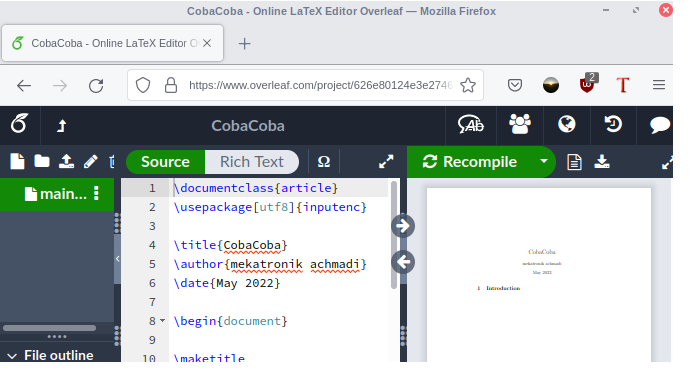
\includegraphics[width=400pt]{images/overleaf}
		\caption{Contoh online editor Overleaf}
	\end{figure}

	\section{Acuan Panduan}

	Untuk kebutuhan panduan disini, digunakan TeXLive offline dengan editor TexStudio di GNU/Linux (ArchLinux) sebagai acuan.
	Anda dapat mengikuti tutorial ini jika anda menggunakan Windows tanpa perlu ada penyesuaian apa pun.

	\bigskip

	Untuk editor online, anda tetap dapat mengikuti dengan sedikit banyak penyesuaian yang mungkin saja tidak dijelaskan di panduan ini.

	\chapter{Dasar Dokumen LaTeX}

	Bab ini menjelaskan dasar penulisan dokumen LaTeX yang berlaku secara umum untuk semua jenis dokumen LaTeX.

	\section{Kerangka}

	Berikut dijelaskan kerangka dasar yang membangun suatu dokumen LaTeX.

	\subsection{Pola Struktur}

	Struktur dasar dokumen umumnya seperti berikut:

	\begin{minted}[frame=lines,framesep=2mm,fontsize=\normalsize,bgcolor=LightGray]{latex}
\documentclass{class} % Definisi jenis dokumen

\usepackage{package} % Memanggil paket definisi tambahan

% Pengaturan tambahan di area ini

\begin{document} % awal dokumen

	% konten dokumen di area ini

\end{document} % akhir dokumen
	\end{minted}

	Beberapa pilihan \textbf{class} yang dapat dipakai antara lain:
	\begin{itemize}
		\item \textbf{article}. Untuk dokumen pendek dan artikel/paper. Paling umum digunakan.
		\item \textbf{report}. Untuk dokumen panjang dan jurnal/disertasi.
		\item \textbf{book}. Untuk membuat buku yang memiliki bab (chapter).
		\item \textbf{letter}. Untuk dokumen surat pemberkasan.
		\item \textbf{beamer}. Untuk membuat slide presentasi.
	\end{itemize}

	\subsection{Contoh Minimum}

	Berikut contoh minimum dokumen LaTeX yang dapat dikompilasi ke format PDF.
	Simpan dengan nama \textbf{helloworld.tex}

	\begin{minted}[frame=lines,framesep=2mm,fontsize=\normalsize,bgcolor=LightGray]{latex}
\documentclass{article}

\usepackage[utf8]{inputenc} % encoding input utf8 (wajib)
\usepackage[T1]{fontenc} % encoding huruf latin (wajib)

\begin{document}
	Hello World, LaTeX
\end{document}
	\end{minted}

	\newpage
	\subsection{Kompilasi PDF}

	Berikut beberapa metode kompilasi ke PDF berdasarkan editor yang digunakan.

	\bigskip

	\textbf{PERINGATAN:} Pada langkah ini diasumsikan bahwa paket offline TexLive atau editor online Overleaf telah siap digunakan.

	\subsubsection{TexStudio}

	Kompilasi PDF dapat dilakukan dengan:
	\begin{itemize}
		\item Klik menu \textit{Tools} -> \textit{Build and View}.
		\item Atau tekan tombol \keys{F5}.
		\item Tunggu beberapa saat hingga muncul pesan "Process exited normally".
		\item Dokumen \textbf{helloworld.pdf} akan muncul di folder yang sama.
	\end{itemize}

	\subsubsection{Visual Studio Code}

	Kompilasi PDF dilakukan di terminal VSCode.
	Langkahnya adalah:

	\begin{itemize}
		\item Klik menu \textit{Terminal} -> \textit{New Terminal} (jika belum ada terminal tab terbuka).
		\item Pastikan alamat terminal sama dengan folder tempat berkas tex berada.
		Anda dapat cek keberadaan berkas terminal dengan perintah:
		\begin{minted}[frame=lines,framesep=2mm,fontsize=\normalsize,bgcolor=LightGray]{bash}
$> ls | grep helloworld.tex
		\end{minted}
		\item Masukkan perintah berikut:
	\begin{minted}[frame=lines,framesep=2mm,fontsize=\normalsize,bgcolor=LightGray]{bash}
$> pdflatex -shell-escape -synctex=1 -interaction=nonstopmode helloworld.tex
	\end{minted}
		\item Tunggu beberapa saat hingga muncul pesan "Output written on helloworld.pdf".
		\item Dokumen \textbf{helloworld.pdf} akan muncul di folder yang sama.
	\end{itemize}

	\textbf{TIPS:} Karena kompilasi dilakukan di terminal, jika menggunakan GNU/Linux maka dapat pula menggunakan
	metode Makefile seperti yang dijelaskan sebelumnya.

\end{document}
